% !TEX TS-program = pdflatex
% CV — Baha Eddine Belhaj Mouldi — Full-Stack Developer — Kuwait market version
\documentclass[a4paper,10pt]{article}
\usepackage[utf8]{inputenc}
\usepackage[T1]{fontenc}
\usepackage[scaled=0.94]{helvet}
\renewcommand{\familydefault}{\sfdefault}
\usepackage[left=1.3cm,right=1.3cm,top=0.9cm,bottom=0.9cm]{geometry}
\usepackage{enumitem}
\usepackage{titlesec}
\usepackage{xcolor}
\usepackage{tikz}
\usepackage{graphicx}
\usepackage[hidelinks]{hyperref}
\definecolor{navy}{RGB}{23,54,93}
\pagestyle{empty}
\setlength{\parindent}{0pt}
\setlength{\parskip}{0pt}
\linespread{0.95}
\hypersetup{pdftitle={CV - Baha Eddine Belhaj Mouldi - Full-Stack Developer},pdfauthor={Baha Eddine Belhaj Mouldi},pdfsubject={Full-Stack Development, Security, Kuwait}}
\titleformat{\section}{\normalsize\bfseries\color{navy}}{}{0pt}{\MakeUppercase}[{\vspace{1pt}\color{navy}\hrule height 0.6pt}]
\titlespacing*{\section}{0pt}{5pt}{2.5pt}
\setlist[itemize]{leftmargin=1.2em,label=\textbullet,itemsep=0.5pt,topsep=1pt,parsep=0pt}
\newcommand{\cventry}[4]{\textbf{#1} \hfill \textbf{#4}\\[1pt]#2{\ifx\relax#3\relax\else, #3\fi}\par\vspace{2pt}}
\newcommand{\repolink}[1]{{\small\href{#1}{#1}}\par\vspace{1pt}}
\begin{document}

% =====================================================================
% HEADER (with photo — standard practice for the Kuwait / GCC market)
% =====================================================================
\begin{minipage}[c]{0.78\textwidth}
{\LARGE\bfseries\color{navy} Baha Eddine Belhaj Mouldi}\\[3pt]
{\large Full-Stack Developer --- Security-Oriented \textbar\ Angular \textbar\ React \textbar\ Spring Boot \textbar\ Python}\\[6pt]
\normalsize
Tunis, Tunisia \quad|\quad +216 55 128 982 \quad|\quad \href{mailto:bahaeddine.belhajmouldi@gmail.com}{bahaeddine.belhajmouldi@gmail.com}\\[2pt]
\href{https://www.linkedin.com/in/bahamouldi}{linkedin.com/in/bahamouldi} \quad|\quad \href{https://github.com/bahamouldi}{github.com/bahamouldi} \quad|\quad \href{https://bahamouldi.github.io/portfolio/}{bahamouldi.github.io/portfolio}\\[3pt]
\textbf{Nationality:} Tunisian \quad|\quad \textbf{Visa status:} Valid Tunisian passport, no Kuwait visa currently held --- available for employer-sponsored work visa (Article 18) \quad|\quad \textbf{Availability:} Immediate / Relocation to Kuwait
\end{minipage}\hfill
\begin{minipage}[c]{0.18\textwidth}
\raggedleft
\begin{tikzpicture}
\clip (0,0) circle (1.25cm);
\node at (0,0) {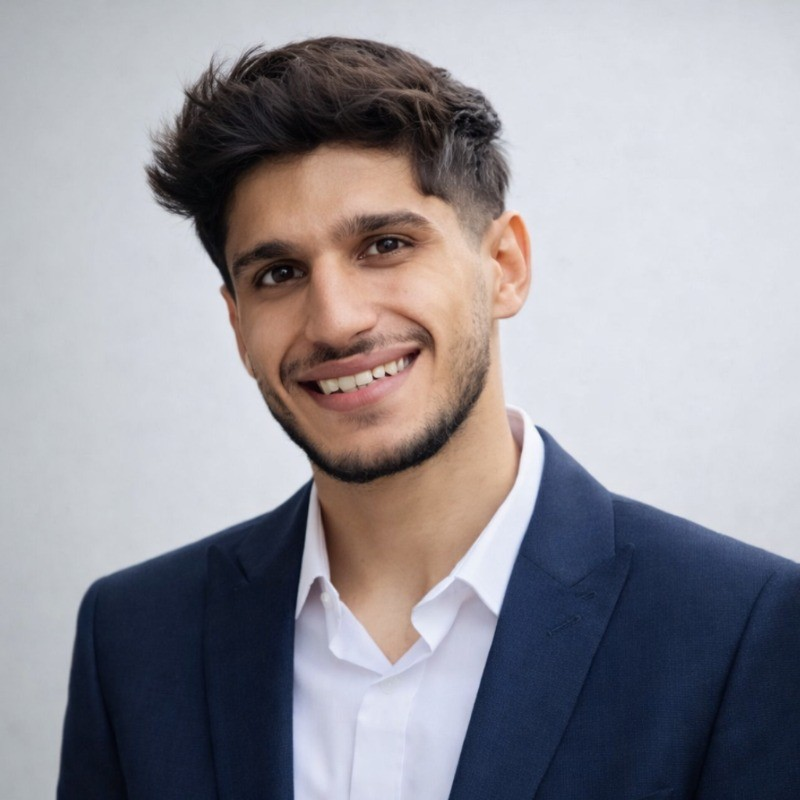
\includegraphics[width=2.6cm,height=2.6cm,keepaspectratio]{photo.jpg}};
\draw[navy,line width=1.4pt] (0,0) circle (1.24cm);
\end{tikzpicture}
\end{minipage}

\vspace{4pt}
\noindent\textcolor{navy}{\rule{\linewidth}{0.8pt}}
\vspace{3pt}

% =====================================================================
\section{Profile}
Computer engineering graduate (ENIT, class of 2026) with hands-on full-stack development experience: Angular/React/Next.js frontend and Java/Spring Boot/Python (FastAPI) backend. Delivered 8+ full-stack projects covering REST API design, database architecture, Docker/Kubernetes deployment and CI/CD pipelines. Built and deployed BeeWAF, a production-grade intelligent Web Application Firewall (10,000+ detection rules, 3 ML models, 98.2\% precision) on a Kubernetes cluster with a full DevSecOps pipeline --- a differentiating combination of full-stack engineering and applied security rarely found in junior profiles. Seeking a Full-Stack Developer role in Kuwait to build secure, high-performance web applications.

% =====================================================================
\section{Core Skills}
\textbf{Frontend} : Angular, React, Next.js, TypeScript, HTML5/CSS3, Tailwind CSS, responsive mobile-first design\\[1pt]
\textbf{Backend} : Java, Spring Boot, Python, FastAPI, Node.js, REST APIs, microservices, JWT/OAuth2 authentication\\[1pt]
\textbf{Databases} : PostgreSQL, MySQL, MongoDB, Prisma ORM, SQL, NoSQL, data modeling\\[1pt]
\textbf{DevOps \& Cloud} : Docker, Kubernetes, Jenkins, ArgoCD (GitOps), GitHub Actions, CI/CD, Prometheus/Grafana, Linux, Bash\\[1pt]
\textbf{Security} : OWASP Top 10, secure coding, penetration testing, WAF engineering, vulnerability remediation\\[1pt]
\textbf{Quality} : Unit \& integration testing, code review, modular architecture, technical documentation

% =====================================================================
\section{Professional Experience}
\cventry{Full-Stack Developer --- Intern (PFE)}{Digital Power Consulting}{Tunisia}{01/2026 -- 05/2026}
\begin{itemize}
  \item Designed and built \textbf{BeeWAF}, an enterprise-grade intelligent Web Application Firewall, end-to-end: FastAPI backend, 10,041 detection rules, 3 ML models (RandomForest, GradientBoosting, IsolationForest), achieving 98.2\% precision with 0\% false positives on test datasets.
  \item Deployed the full application to production on a Kubernetes cluster (3 masters + 2 workers, Calico CNI): complete manifests (Deployment, Service, Ingress, PVC), health/liveness probes, zero-downtime rolling updates.
  \item Built the CI/CD pipeline: Jenkins (8 stages) + ArgoCD (GitOps), with Prometheus/Grafana monitoring dashboards and ELK-based real-time alerting.
  \item Implemented 27 security modules (anti-bot, DLP, anti-DDoS, virtual patching of 37 CVEs) achieving compliance with 7 frameworks (OWASP, PCI DSS, GDPR, NIST, ISO 27001, CIS, SOC 2).
\end{itemize}
\cventry{Full-Stack Developer, Freelance (Part-Time)}{Digital Power Consulting}{Tunisia}{01/2025 -- 12/2025}
\begin{itemize}
  \item Built full-stack web applications for clients: Angular/TypeScript frontend, Java/Spring Boot backend, REST APIs, PostgreSQL/MySQL databases.
  \item Designed responsive user interfaces, integrated authentication systems (JWT, OAuth2), Docker containerization and CI/CD deployment.
  \item Performed penetration testing on 8 web and API applications, delivering detailed remediation reports for clients.
\end{itemize}
\cventry{Cybersecurity Intern --- SAP Threat Detection}{Streamlink}{Tunisia}{07/2025 -- 08/2025}
\begin{itemize}
  \item Built an automated SAP threat detection pipeline (Python/RFC SDK $\rightarrow$ ELK $\rightarrow$ N8N $\rightarrow$ TheHive) with detection under 2 minutes and auto-blocking under 7 minutes, 0\% false positives.
  \item Monitored sensitive SAP transactions and configured real-time Kibana dashboards for security alerting.
\end{itemize}
\cventry{Network Security Intern}{Tunisie Telecom}{Tunisia}{07/2024}
\begin{itemize}
  \item Built network monitoring dashboards (Elastic/Kibana), analyzed traffic data and identified 10+ vulnerabilities.
\end{itemize}

% =====================================================================
\section{Full-Stack Projects}
\cventry{BeeWAF --- Intelligent Web Application Firewall (PFE, graded 86/100)}{FastAPI, Python, ML, Docker, Kubernetes, ELK, Prometheus, Grafana}{}{2026}
\begin{itemize}
  \item Enterprise WAF deployed in production: 27-module inspection pipeline, 107 signatures (9,824 regex patterns), 18-layer evasion detection.
  \item ML evaluation on the CSIC 2010 dataset (12,213 requests): 92.3\% accuracy, 98.2\% precision, 89.8\% F1-score; production latency overhead under 20ms (median).
  \item MITRE ATT\&CK mapping (22 techniques) with APT-group attribution (APT28, APT29, Lazarus).
\end{itemize}
\repolink{https://github.com/bahamouldi/beewaf\_final}
\cventry{Fedi Phone --- E-commerce Platform}{Next.js, TypeScript, React, Prisma, PostgreSQL, Tailwind CSS, Docker}{}{2026}
\begin{itemize}
  \item Complete full-stack e-commerce: REST API backend, JWT authentication, cart, wishlist, real-time search, admin dashboard, WhatsApp order integration, Prisma ORM, dark mode.
\end{itemize}
\repolink{https://github.com/bahamouldi/Fedi\_Phone}
\cventry{Revenue Assurance Dashboard --- Tunisie Telecom}{Python, Streamlit, PostgreSQL, Plotly, RAG}{}{2026}
\begin{itemize}
  \item Star-schema data warehouse analyzing ~900,000 telecom revenue records (Q1 2025 -- Q1 2026) across 4 domains (Voice/SMS, Data, Recharge, SMS Plus), with a RAG chatbot and 3--30 day forecasting dashboards.
\end{itemize}
\repolink{https://github.com/bahamouldi/tunisie\_telecom}
\cventry{Financial Analysis Platform --- SFBT}{Python, Data Warehouse, BI, ML}{}{2026}
\begin{itemize}
  \item Complete ETL pipeline computing 20,000+ automated financial ratios (MSI 20000 standard), with BI dashboards and predictive models.
\end{itemize}
\repolink{https://github.com/bahamouldi/pfe\_malik}
\cventry{IDTS \& Kairos --- Secure Enterprise Platforms}{Java, Spring Boot, Angular, PostgreSQL, Docker, Kubernetes}{}{2024}
\begin{itemize}
  \item Two full-stack applications: Spring Boot REST backends (JPA), Angular frontends, PostgreSQL, Docker/Kubernetes deployment.
\end{itemize}
\cventry{Microservices Architecture}{TypeScript, Node.js, REST API, Docker}{}{2026}
\begin{itemize}
  \item Distributed microservices application: decoupled services, REST communication, modular organization.
\end{itemize}
\repolink{https://github.com/bahamouldi/microservise}

% =====================================================================
\section{Education}
\cventry{Engineering Degree in Computer Science}{National Engineering School of Tunis (ENIT)}{Tunisia}{09/2023 -- 06/2026}
\begin{itemize}
  \item Graduated 06/25/2026 following the defense of the final-year (PFE) project.
  \item Ranked 65\textsuperscript{th} out of 600+ candidates in the national engineering school entrance exam.
\end{itemize}
\cventry{Preparatory Classes (Physics \& Technology)}{Preparatory Institute for Engineering Studies, El Manar}{Tunisia}{09/2021 -- 06/2023}
\cventry{Technical Baccalaureate --- Distinction (Mention Tr\`es Bien)}{Lyc\'ee Abdelaziz Khouja, K\'elibia}{Tunisia}{06/2021}

% =====================================================================
\section{Certifications}
Git \& GitHub --- 365 Data Science (2024) ; Networking --- Cisco (2025) ; Fundamentals of Deep Learning --- NVIDIA (2025) ; Exploring Adversarial Machine Learning --- NVIDIA (2025) ; Machine Learning --- NVIDIA (2024).

% =====================================================================
\section{Languages}
French (Fluent) \quad|\quad English (B2) \quad|\quad Arabic (Native) \quad|\quad Chinese (Basic)

% =====================================================================
\section{References}
Available upon request.

\end{document}
